\appendix
\chaptermark{}
\section{Supplementary for Chapter 3}

\subsection{Derivation of the Frobenius norm identity} \label{app:frobenius}
Recall $a \in \R^{B\times T \times d}$ is the input to a linear layer with weight matrix $W \in \R^{p \times d}$, and $g \in \R^{B \times T \times p}$ is the gradient of the loss w.r.t. the output. The identity follows from trivial algebra:
\eqn{
\normf{ \nabla_W \mathcal{L}_i }^2 = \normf{ g_i^\top a_i }^2
&= \normf{ \sum_{k=1}^T g_{i, k} a_{i, k}^\top }^2 \\
&=
    \sum_{r=1}^d \sum_{s=1}^p \bracks{
        \sum_{k=1}^T a_{i, k, r} g_{i, k, s}
    }^2 \\
&=
    \sum_{r=1}^d \sum_{s=1}^p \sum_{k_1=1}^T \sum_{k_2=1}^T 
        a_{i, k_1, r} g_{i, k_1, s}
        a_{i, k_2, r} g_{i, k_2, s} \\
&=
    \sum_{k_1=1}^T \sum_{k_2=1}^T
        \bracks{ \sum_{r=1}^d a_{i, k_1, r} a_{i, k_2, r} }
        \bracks{ \sum_{s=1}^p g_{i, k_1, s} g_{i, k_2, s} } \\
&=
    \mathrm{vec}(a_{i} a_{i}^\top)^\top \mathrm{vec}( g_i g_i^\top ). 
}
Note that when $T=1$, the identity takes the form of 
\eqn{
\normf{ \nabla_W \mathcal{L}_i }^2
= 
    \mathrm{vec}(a_{i} a_{i}^\top)^\top \mathrm{vec}( g_i g_i^\top )
= 
    \normtwo{a_i}^2 \normtwo{g_i}^2. 
}
This is the \cite{goodfellow2015efficient} trick.

\newpage
\subsection{Experiment Details}\label{app:experiments_main}

\paragraph{Sentence Classification.}
Results for RGP in Table~\ref{table:glue} are taken from documented numbers in their released codebase.\footnote{\url{https://github.com/dayu11/Differentially-Private-Deep-Learning/tree/main/language}}
These results are under the DP guarantees of $(\epsilon, \delta)=(3, 10^{-5})$ or $(\epsilon, \delta)=(8, 10^{-5})$.
These guarantees are strictly looser than our guarantees which are based on $\delta=\nicefrac{1}{2 |\D_\text{train}|}$ (recall the smallest dataset in this cohort of tasks has $60$k+ records).
The RGP numbers in Table~~\ref{table:glue} are higher than those reported in their paper~\citep{yu2021large}, since the latter numbers are not based on fine-tuning the official RoBERTa models.

\paragraph{Table-To-Text Generation.}
To evaluate models trained on E2E and DART, we evaluate generations from models obtained with beam search with a beam size of $5$.
For evaluation, we run the official pipeline for E2E,\footnote{\url{https://github.com/tuetschek/e2e-metrics}} and the pipeline used in the GEM benchmark~\citep{gehrmann2021gem} for DART.\footnote{\url{https://github.com/GEM-benchmark/GEM-metrics}}

\paragraph{Chit-Chat Dialog Generation.}
We built off Huggingface's codebase of the winning entry of the ConvAI2 competition,
\footnote{\url{https://github.com/huggingface/transfer-learning-conv-ai}}
\footnote{\url{http://convai.io/2018/}} and used their preprocessed training set with the minor modification of truncating the number of training examples to be a multiple of the batch size.
The original ConvAI2 competition is aimed at advancing research on building engaging chatbots and also requested models to predict the mostly likely response given a list of candidates.
The challenge included hits@1 as part of its suite of automatic metrics.
For simplicity, we skip this step of predicting the most likely response for both training and evaluation. 
Results for the entry HuggingFace (ConvAI2 winner) in Table~\ref{table:personachat} are taken from the official validation set leader board.\footnote{\url{https://github.com/DeepPavlov/convai/blob/master/leaderboards.md}}
Our reimplementation of HuggingFace's submission uses the released code for their winning entry, fine-tunes GPT with the default hyperparameters, and removes the classification loss for learning to predict the most likely response given candidates.

We additionally fine-tuned DialoGPT-medium~\citep{zhang2019dialogpt}, since the model was pretrained on conversation-like exchanges extracted from Reddit comment chains. Intuitively, this pretraining corpus is more aligned with the downstream fine-tuning data than WebText~\citep{radford2019language}, and thus would likely improve downstream performance.

To evaluate the F1 score, we obtained predicted responses from trained models using beam search with a beam size of $5$.
Since past work found that the F1 score can be gamed by always letting the model predict a predetermined phrase~\citep{dinan2019second}, we additionally ask humans to rate generations from the model through Amazon mechanical turk to obtain a more complete picture of model quality.
When sampling responses for human evaluation, we used nucleus sampling with $p=0.9$~\citep{holtzman2019curious}.
For human evaluation, we asked 20 turkers to each rate 5 entries.
For each entry, a turker is asked to rate on a scale of 1 to 5 the quality of predicted responses from privately fine-tuned DialoGPT-medium models, non-privately fine-tuned DialoGPT-medium models, non-privately fine-tuned GPT models (our reimplementation of HuggingFace's entry), and the reference text, given the history of the dialog. 
Since human evaluation can yield noisy results, we also report the $95\%$ asymptotic confidence interval in Table~\ref{table:personachat}.
All models were trained and evaluated on the version of Persona-Chat with the original persona.
All numbers reported in Table~\ref{table:personachat} are obtained on the validation split. 

\newpage
\subsection{Subtleties of implementing DP mixed precision training}
\label{app:mixed_precision}
Mixed precision training~\citep{micikevicius2017mixed} accelerates updates by storing certain tensors in half-precision.
To mitigate negative effects caused by potential arithmetic underflow, usual implementations upscale the loss with an adaptive factor pre-backpropagation and downscale the gradients with the same factor post-backpropagation. 
The scaling factor is adapted based on whether underflow is observed during training.

Special care needs to be taken when combining gradient privatization with mixed precision training.
One implementation that ensures similar results across full and mixed precision training 
(1) upscales the loss with the adaptive factor $K$, (2) clips per-example gradients by $C K$, (3) adds to the sum of clipped gradients the usual Gaussian noise multiplied by $K$, and (4) downscales the noisy gradient by $K$.
This is the implementation that we adopt, and we were able to obtain similar results on the E2E dataset with and without mixed precision. 

One alternative implementation (a) upscales the loss with the adaptive factor $K$, (b) clips per-example gradients by $C$, (c) adds the usual Gaussian noise to the sum of clipped gradients, and (d) downscales noisy gradients by $K$. 
The main difference between this procedure and the prior is whether the factor $K$ is considered during clipping and noising.
This procedure, while having the same DP guarantee, typically does not result in similar results as full precision when the same hyperparameters are used across the two settings (even with an optimizer like Adam which self-adjusts the magnitude of updates with accumulated empirical second moments).
We also identified that this implementation is also the primary reason that a prior work's code does not produce good results with full fine-tuning using our near-optimal hyperparameters.\footnote{
    \url{https://github.com/dayu11/Differentially-Private-Deep-Learning}
}

\newpage
\subsection{Hyperparameter Search Ranges}\label{app:hp_search_range}
We compare different adaptation methods by reporting task specific metrics on the test split using hyperparameters that maximize validation BLEU on E2E.
For sentence classification tasks, we reused the same hyperparameters, except for the number of training epochs and batch size.
For SST-2, we reused the same batch size as for private E2E fine-tuning, and the number of epochs exactly as in typical non-private fine-tuning for SST-2 (number of epochs equals to 3 in this case).
For remaining classification tasks, we use a batch size such that the sampling rate is the same as for SST-2, and a number of training epochs that is roughly proportional to the dataset size.
Appendix~\ref{app:hp_transfer} outlines why we transfer the sampling rate as opposed to the batch size.
We list the range of hyperparameters that we searched over for each individual adaptation method on E2E considered in the paper. 
Prefix-tuning has two additional hyperparameters: the length of the prefix and the dimensionality of the hidden layer. 
We set these to the default used by~\cite{li2021prefix} (10 for the former and 512 for the latter).
For Adam, we use the default hyperparamaters set by PyTorch~\citep{paszke2017automatic}. 

\begin{table}[H]
    \centering
    \footnotesize
    \setlength{\tabcolsep}{0.7pt}
    \renewcommand{\arraystretch}{1.2}
    \caption{Hyperparameter search range for different methods.}
    \begin{tabular}{@{} l c c c c @{}}
        \toprule
        Method & Full & Prefix & Linear & FT2\\
        \midrule
        Guarantee $(\epsilon, \delta)$ &
        $(3, \nicefrac{1}{2|\mathcal{D}_{\text{train}}|})$ & 
        $(3, \nicefrac{1}{2|\mathcal{D}_{\text{train}}|})$ & 
        $(3, \nicefrac{1}{2|\mathcal{D}_{\text{train}}|})$ & 
        $(3, \nicefrac{1}{2|\mathcal{D}_{\text{train}}|})$ \\
        Clipping norm $C$ &0.1 & 0.1 & 0.1 & 0.1\\
        Batch size $B$ 
        &$\{512, 1024\}$ 
        &$\{512, 1024\}$ 
        &$\{512, 1024\}$
        &$\{512, 1024\}$\\
        Learning rate $\eta$
        & \tiny $ \{200, 100, 30, 10, 3\} \cdot 10^{-5}$
        & \tiny $\{200, 100, 30, 10, 3\} \cdot 10^{-5}$
        & \tiny $\{200, 100, 30, 10, 3\} \cdot 10^{-5}$
        & \tiny $\{200, 100, 30, 10, 3\} \cdot 10^{-5}$ \\
        LR decay
        & $\{ \text{yes}, \text{no}\}$ 
        & $\{ \text{yes}, \text{no}\}$ 
        & $\{ \text{yes}, \text{no}\}$ 
        & $\{ \text{yes}, \text{no}\}$ \\
        Epochs $E$
        &$\{10, 30, 50\}$
        & $\{10, 30, 50\}$
        & $\{10, 30, 50\}$
        & $\{10, 30, 50\}$ \\
        Weight decay $\lambda$ & 0 & 0 & 0 & 0 \\
        Noise scale $\sigma$ 
        & \multicolumn{4}{c}{calculated numerically based on $(\epsilon, \delta)$-DP budget} \\
        \bottomrule
        \end{tabular}
        \label{tab:hparams}
\end{table}

\begin{table}[H]
    \centering
    \setlength{\tabcolsep}{7pt}
    \renewcommand{\arraystretch}{1.2}
    \caption{Hyperparameter search range for different methods (continued).}
    \begin{tabular}{@{} l c c @{}}
        \toprule
        Method & LoRA & RGP \\
        \midrule
        DP guarantee $(\epsilon, \delta)$ &
        $(3, \nicefrac{1}{2|\mathcal{D}_{\text{train}}|})$ & 
        $(3, \nicefrac{1}{2|\mathcal{D}_{\text{train}}|})$ \\
        Clipping norm $C$ &0.1 & $\{ 0.1, 1, 10\}$ \\
        Batch size $B$ 
        &$\{512, 1024\}$ 
        &$\{512, 1024\}$ \\
        Learning rate $\eta$ & 
        $ \{300, 100, 30, 10, 3\} \cdot 10^{-5}$ & 
        $\{300, 100, 30, 10, 3\} \cdot 10^{-5}$ \\
        LR decay
        & $\{ \text{yes}, \text{no}\}$ 
        & $\{ \text{yes}, \text{no}\}$ \\
        Epochs $E$
        &$\{5, 10, 30, 50\}$
        & $\{5, 10, 30, 50\}$\\
        Weight decay $\lambda$ & 0 & 0 \\
        Rank $k$ 
        &$\{1,2, 4,8\}$ & $\{1,2,4, 8\}$ \\
        Noise scale $\sigma$ & 
        \multicolumn{2}{c}{calculated numerically based on $(\epsilon, \delta)$-DP budget} \\
        \bottomrule
        \end{tabular}
        \label{tab:hparams_low_rank}
\end{table}


\newpage
\subsection{Uncurated Samples from fine-tuned models}\label{app:samples}

\begin{table}[h]
\centering
\renewcommand{\arraystretch}{0.7}
\scriptsize
\begin{tabular}{l | p{0.8\linewidth}}
\toprule
Table & name : The Punter | Type : restaurant | food : Indian | price : cheap | customer rating : average | area : riverside | family friendly : no | near : Express by Holiday Inn  \\
 \hline
GPT-2 $(\epsilon=3)$ & The Punter is a cheap Indian restaurant near Express by Holiday Inn in the riverside area. It is not family - friendly. \\
GPT-2 $(\epsilon=8)$ & The Punter is a cheap Indian restaurant near Express by Holiday Inn in the riverside area. It is not family - friendly. \\
GPT-2-m $(\epsilon=3)$ & The Punter is a cheap Indian restaurant located in the riverside area near Express by Holiday Inn. It has an average customer rating and is not family - friendly. \\
GPT-2-m $(\epsilon=8)$ & The Punter is a restaurant providing Indian food in the cheap price range. It is located in the riverside area near Express by Holiday Inn. Its customer rating is average. \\
GPT-2-l $(\epsilon=3)$ & The Punter is a cheap Indian restaurant in the riverside area near Express by Holiday Inn. It is not family - friendly and has an average customer rating. \\
GPT-2-l $(\epsilon=8)$ & The Punter is a restaurant providing Indian food in the cheap price range. It is located in the riverside area near Express by Holiday Inn. Its customer rating is average. \\
\hline
 Reference & The restaurant named The Punter has cheap Indian food and an average customer rating . It is near the Express by Holiday Inn on the riverside and is not family friendly . \\
\midrule\midrule
Table & name : The Mill | Type : restaurant | food : English | price : moderate | customer rating : 3 out of 5 | area : city centre | family friendly : yes | near : Café Rouge  \\
 \hline
GPT-2 $(\epsilon=3)$ & The Mill is a moderately priced restaurant located in the city centre near Café Rouge. \\
GPT-2 $(\epsilon=8)$ & The Mill is a moderately priced restaurant located in the city centre near Café Rouge. \\
GPT-2-m $(\epsilon=3)$ & The Mill is an English restaurant located in the city centre near Café Rouge. It is moderately priced and has a customer rating of 3 out of 5. \\
GPT-2-m $(\epsilon=8)$ & The Mill is a moderately priced restaurant located in the city centre near Café Rouge. It is child friendly and has a customer rating of 3 out of 5. \\
GPT-2-l $(\epsilon=3)$ & The Mill is a moderately priced English restaurant in the city centre near Café Rouge. It is child friendly and has a customer rating of 3 out of 5. \\
GPT-2-l $(\epsilon=8)$ & The Mill is a kid friendly English restaurant in the city centre near Café Rouge. It has a moderate price range and a customer rating of 3 out of 5. \\
\hline
 Reference & Serving moderately priced English food with a 3 out of 5 customer approval , The Mill restaurant is kid friendly and conveniently located at the city centre near the Café Rouge . \\
\midrule\midrule
Table & name : The Vaults | Type : pub | food : Japanese | price : high | customer rating : 3 out of 5 | area : city centre | family friendly : yes | near : Raja Indian Cuisine  \\
 \hline
GPT-2 $(\epsilon=3)$ & Located near Raja Indian Cuisine in the city centre, The Vaults is a family - friendly Japanese pub with a high customer rating. \\
GPT-2 $(\epsilon=8)$ & The Vaults is a Japanese pub in the city centre near Raja Indian Cuisine. It has a high price range and a customer rating of 3 out of 5. \\
GPT-2-m $(\epsilon=3)$ & The Vaults is a Japanese pub located in the city centre near Raja Indian Cuisine. It has a high price range and a customer rating of 3 out of 5. \\
GPT-2-m $(\epsilon=8)$ & The Vaults is a Japanese pub located in the city centre near Raja Indian Cuisine. It has a high price range and a customer rating of 3 out of 5. \\
GPT-2-l $(\epsilon=3)$ & The Vaults is a Japanese pub in the city centre near Raja Indian Cuisine. It has a high price range and a customer rating of 3 out of 5. \\
GPT-2-l $(\epsilon=8)$ & The Vaults is a child friendly Japanese pub in the city centre near Raja Indian Cuisine. It has a high price range and a customer rating of 3 out of 5. \\
\hline
 Reference & Located near the Raja Indian Cuisine at the city centre , is family - friendly pub The Vaults . Serving Japanese food , The Vaults , is high priced with a 3 out of 5 customer satisfaction rating . \\
\bottomrule
\end{tabular}
\vspace{-2mm}
\caption{\small Full fine-tuned GPT-2, GPT-2-m, and GPT-2-l generations on E2E test split.}
\end{table}


\begin{table}[h]
\centering
\renewcommand{\arraystretch}{1.2}
\scriptsize
\begin{tabular}{l | p{0.8\linewidth}}
\toprule
Table & Real Madrid Castilla : manager : Luis Miguel Ramis | Abner (footballer) : club : Real Madrid Castilla | Abner (footballer) : club : C.D. FAS  \\
 \hline
GPT-2 $(\epsilon=3)$ & Luis Miguel Ramis played for Real Madrid Castilla and played for C.D. FAS. \\
GPT-2 $(\epsilon=8)$ & Luis Miguel Ramis is the manager of Abner (footballer) who plays for Real Madrid Castilla. \\
GPT-2-m $(\epsilon=3)$ & Luis Miguel Ramis is the manager of Real Madrid Castilla. He plays for C.D. FAS. \\
GPT-2-m $(\epsilon=8)$ & Luis Miguel Ramis is the manager of Real Madrid Castilla. He plays for C.D. FAS. \\
GPT-2-l $(\epsilon=3)$ & Luis Miguel Ramis is the manager of Real Madrid Castilla and C.D. FAS. \\
GPT-2-l $(\epsilon=8)$ & Luis Miguel Ramis is the manager of Real Madrid Castilla and Abner (footballer) plays for C.D. FAS. \\
\hline
 Reference & Footballer, Abner, plays C.D. FAS. and Real Madrid Castilla, the manager of which, is Luis Miguel Ramis. \\
\midrule\midrule
Table & United States : ethnic\_group : Asian Americans | United States : capital : Washington, D.C. | Albany, Oregon : is\_part\_of : Benton County, Oregon | Albany, Oregon : country : United States  \\
 \hline
GPT-2 $(\epsilon=3)$ & The capital of the United States is Washington, D.C. and is part of Benton County, Oregon. \\
GPT-2 $(\epsilon=8)$ & The capital of the United States is Washington, D.C. and is part of Benton County, Oregon. \\
GPT-2-m $(\epsilon=3)$ & Albany, Oregon is part of Benton County, Oregon in the United States where Asian Americans are an ethnic group. \\
GPT-2-m $(\epsilon=8)$ & Albany, Oregon is part of Benton County, Oregon in the United States where Asian Americans are an ethnic group. \\
GPT-2-l $(\epsilon=3)$ & Albany, Oregon is part of the United States where Asian Americans are an ethnic group and the capital is Washington D.C. \\
GPT-2-l $(\epsilon=8)$ & Albany, Oregon is part of the United States where Asian Americans are an ethnic group and the capital is Washington D.C. \\
\hline
 Reference & The Asian Americans are an ethnic group in the United States, which has the capital city of Washington DC. It is also the location of Albany, part of Benton County in Oregon. \\
\midrule\midrule
Table & A Loyal Character Dancer : language : English language | English language : spoken\_in : Great Britain | A Loyal Character Dancer : country : United States | United States : ethnic\_group : Native Americans in the United States  \\
 \hline
GPT-2 $(\epsilon=3)$ & A Loyal Character Dancer is an English language spoken in the United States where Native Americans are the ethnic group. \\
GPT-2 $(\epsilon=8)$ & A Loyal Character Dancer is written in English and is spoken in Great Britain. Native Americans are an ethnic group in the United States. \\
GPT-2-m $(\epsilon=3)$ & A Loyal Character Dancer is written in English and is written in the United States where Native Americans are an ethnic group. \\
GPT-2-m $(\epsilon=8)$ & A Loyal Character Dancer is written in English and is written in the United States where Native Americans are an ethnic group. \\
GPT-2-l $(\epsilon=3)$ & A Loyal Character Dancer is written in English and is written in the United States where Native Americans are an ethnic group. \\
GPT-2-l $(\epsilon=8)$ & A Loyal Character Dancer is written in English, which is spoken in Great Britain and the United States. Native Americans are an ethnic group in the United States. \\
\hline
 Reference & A Loyal Character Dancer is written in English which is spoken in Great Britain. The book is published in the United States where the Native Americans are an ethnic group. \\
\bottomrule
\end{tabular}
\caption{\small Full fine-tuned GPT-2, GPT-2-m, and GPT-2-l generations on DART test split.}
\end{table}


\begin{table}[h]
\centering
\renewcommand{\arraystretch}{1.2}
\scriptsize
\begin{tabular}{l | p{0.8\linewidth}}
\toprule
Persona & ['i am 40 years old.', 'i work as a car salesman.', 'my wife spends all my money.', 'i hate my job.', "i'm planning on getting a divorce."] \\
 \hline
History & ['i know the struggle, i volunteer at a homeless shelter', "great, i hope you don't get to see me there.", 'i hope not either, would not wish it on my worse enemy', 'between wife, job with no money, i am thinking now of divorce.', "i've given it a few thoughts before"] \\
 \hline
GPT-2-m $(\epsilon=3)$ & i wish i had a better idea . \\
GPT-2-m $(\epsilon=8)$ & i think i will . what are your thoughts on divorce ? \\
DialoGPT-medium $(\epsilon=3)$ & i'm sorry to hear that . i hope you don't have any financial problems . \\
DialoGPT-medium $(\epsilon=8)$ & i don't have any money , i do not know how i could manage . \\
\hline
 Reference & do you give demonstrations of your skills ? \\
\midrule\midrule
Persona & ['my mother is a dentist.', 'my favourite artist is travis scott.', 'i have one older sister.', 'i am currently looking for a job preferably at a restaurant.', 'i like playing basketball.'] \\
 \hline
History & ['hello, how are you tonight?'] \\
 \hline
GPT-2-m $(\epsilon=3)$ & i'm good , good luck \\
GPT-2-m $(\epsilon=8)$ & i am good , just listening to travis scott . what about you ? \\
DialoGPT-medium $(\epsilon=3)$ & i'm good . just got back from a dentist visit . \\
DialoGPT-medium $(\epsilon=8)$ & i am doing well . just got back from a dentist visit \\
\hline
 Reference & i am good . about to go to basketball practice . \\
\midrule\midrule
Persona & ['my mom passed away when i was young.', 'i work in the insurance business.', 'my father is in the army.', 'i recently was fired and had to get a new job.'] \\
 \hline
History & ["god isn't really real", 'to each their own, but i believe he is.', 'my children are gone now', 'i lost my mom at a young age', 'my wife took them all'] \\
 \hline
GPT-2-m $(\epsilon=3)$ & she was a great mother \\
GPT-2-m $(\epsilon=8)$ & they were so young , they were so crazy \\
DialoGPT-medium $(\epsilon=3)$ & that is horrible . my mom was a soldier \\
DialoGPT-medium $(\epsilon=8)$ & what happened to her ? \\
\hline
 Reference & sorry to hear that . i barely see my dad he's in the army \\
\midrule\midrule
Persona & ['i am also a graduate student.', 'i walk dogs for a living.', 'my parents taught me survival skills.', 'i am an avid kayaker.', 'i enjoy reading journals and guides related to psychology.'] \\
 \hline
History & ['hi, how are you today?', "good evening. how are you tonight? i'm well.", 'i am doing good, i just finished playing ping pong.', 'i am trying to write invoices for my dog walking business.', 'that seems like hare work, i like to play the violin in my free time.'] \\
 \hline
GPT-2-m $(\epsilon=3)$ & i have a lot of dogs , i walk them on my walks . \\
GPT-2-m $(\epsilon=8)$ & that is a very rewarding hobby . i have a dog named jasper . \\
DialoGPT-medium $(\epsilon=3)$ & oh , that is a nice hobby . what do you do for a living ? \\
DialoGPT-medium $(\epsilon=8)$ & it is . i love learning to play the violin . \\
\hline
 Reference & i love the violin . i do not play anything . i kayak for fun however . \\
\bottomrule
\end{tabular}
\caption{\small Full fine-tuned GPT-2-m and DialoGPT-m generations on Persona-Chat val split.}
\end{table}

\clearpage
\newpage
\section{Supplementary for Chapter 4}


\subsection{Additional Experiments on Run Time}
\label{app:runtime}

We include additional experiments comparing the run time of different clipping approaches.
Our goal is to further consolidate the claims that 1) adaptive per-layer clipping attains similar or better task performances under the same epoch budget for certain workflows, and that 2) this translates into compute time savings since per-layer clipping is faster than alternative clipping approaches per update (or almost equivalently per epoch).
All experiments here are performed on a machine with a single Titan RTX GPU with 24 GB of VRAM (different from the configuration in Figure~\ref{fig:throughput-comparison} which uses a single A6000 GPU).

The direct experiment we perform is to full fine-tune GPT-2 on E2E with three clipping approaches (adaptive per-layer, ghost, and flat clipping) under the same epoch constraint (which we fix to be 10 for all workflows).
Regarding hyperparameters for flat clipping, we adopt the set of values obtained from extensive tuning on this task used by~\cite{li2022large}.
We reuse the same set of hyperparameters values for ghost clipping, since the approach essentially results in the same gradient updates as flat clipping up to numerical precision (only computed in a different way).
Using these near optimal hyperparameters for flat and ghost clipping prevents our experiments from unfairly disfavouring the two approaches.
Figure~\ref{fig:gpt2runtime-overall-nll} shows that adaptive per-layer clipping consistently achieves lower test set negative log-likelihood than flat clipping and ghost clipping under any given wall time elapse.
While language generation metrics (e.g., BLEU and ROUGE-L) are generally noiser than the test set NLL, Figure~\ref{fig:gpt2runtime-overall-task-metric} shows that adaptive per-layer clipping generally yields better task metric numbers compared to flat clipping and ghost clipping under the same wall time.

Finally, we note the caveat that the precise run time advantage of adaptive per-layer clipping against flat clipping may vary across machines and GPU types.
In addition, the realized gains for actual training workflows might be smaller than that observed in our controlled experiments (e.g., Figure~\ref{fig:throughput-comparison}) due to compute time spent on auxiliary operations such as data loading and data preprocessing (e.g., pad sequences of different length to the same length). 
For instance, we repeat the controlled experiment in Figure~\ref{fig:throughput-comparison} but this time with a different GPU, and observe slightly different factors of speed gains. 
Overall, we generally see that adaptive per-layer clipping is above 1.4x the speed of flat clipping in our controlled experiments, and the realized gains is roughly as much for full fine-tuning on E2E with our implementation.

\begin{figure}[htb]
\begin{center}
\begin{minipage}[t]{0.5\linewidth}
\centering
{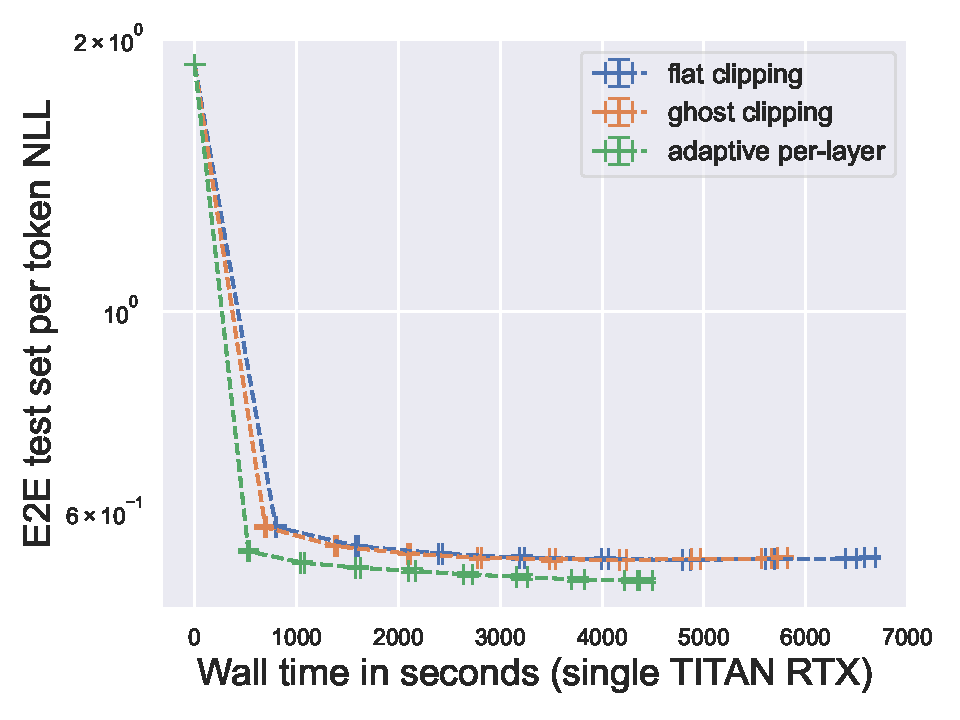
\includegraphics[width=0.95\linewidth]{files/fig/walltime_e2e_test_nll.pdf}} \end{minipage}
\end{center}
\caption{
Adaptive per-layer clipping consistently achieves lower test set negative log-likelihood than flat clipping and ghost clipping under the same wall time.
}
\label{fig:gpt2runtime-overall-nll}
\end{figure}

\begin{figure}[htb]
\begin{center}
\begin{minipage}[t]{0.45\linewidth}
\centering
{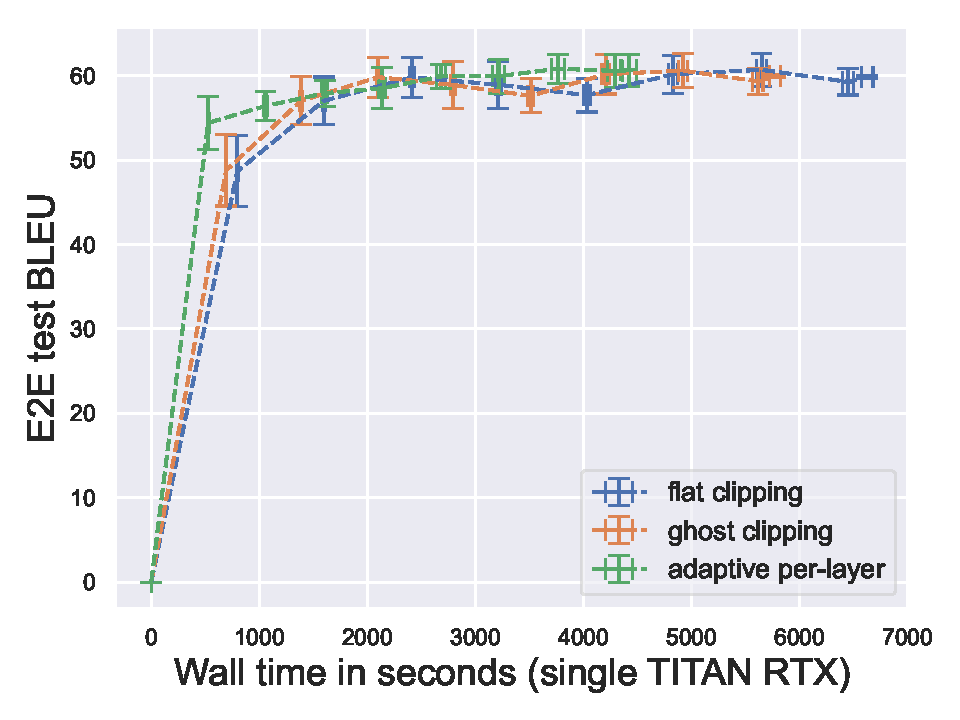
\includegraphics[width=0.95\textwidth]{files/fig/walltime_e2e_test_bleu.pdf}} \\
(a) BLEU
\end{minipage}
\begin{minipage}[t]{0.45\linewidth}
\centering
{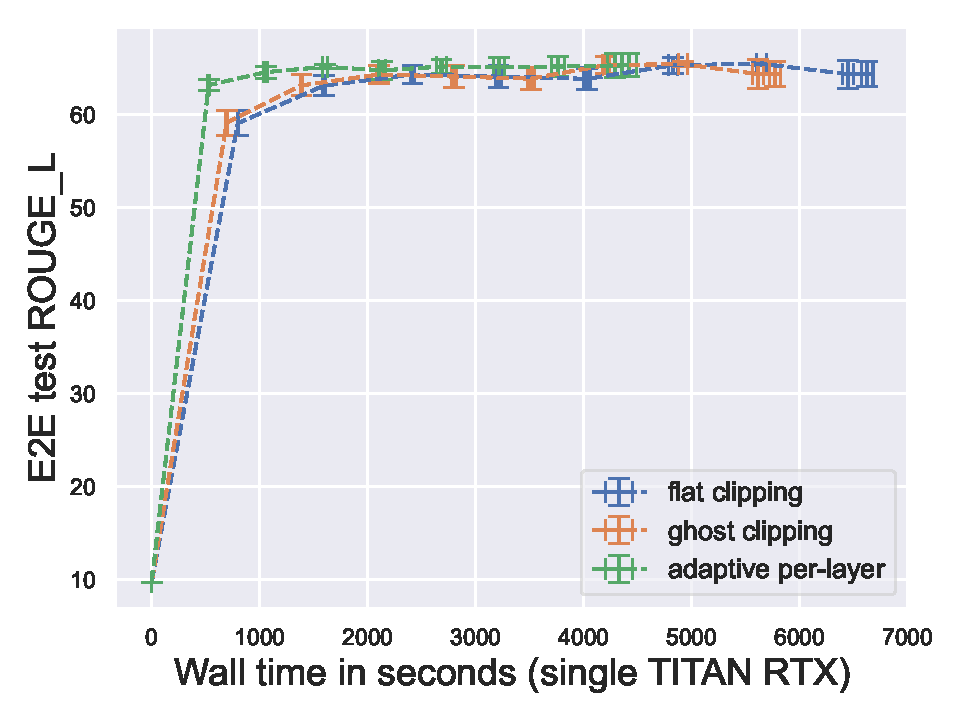
\includegraphics[width=0.95\textwidth]{files/fig/walltime_e2e_test_ROUGE_L.pdf}} \\
(b) ROUGE-L
\end{minipage}
\end{center}
\caption{
Adaptive per-layer clipping generally yields better task metric numbers compared to flat clipping and ghost clipping under the same wall time.
}
\label{fig:gpt2runtime-overall-task-metric}
\end{figure}


\begin{figure}[htb]
\begin{center}
\begin{minipage}[t]{0.45\linewidth}
\centering
{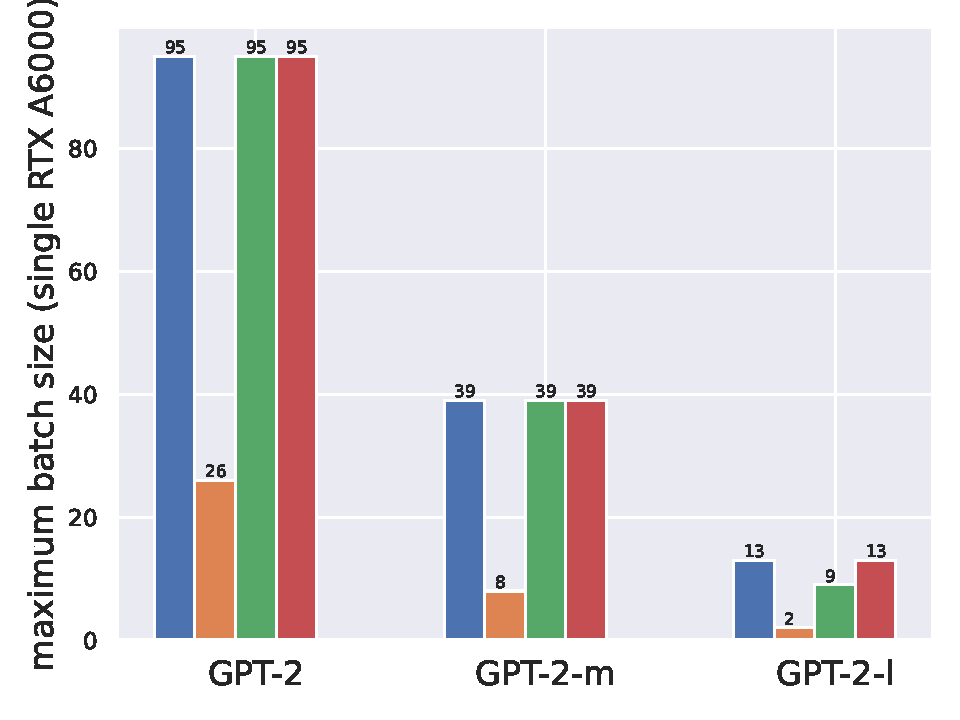
\includegraphics[width=0.95\linewidth]{files/fig/profile_v2/memory_100_default_fast_float.pdf}} \\
(a) Memory
\end{minipage}
\begin{minipage}[t]{0.45\linewidth}
\centering
{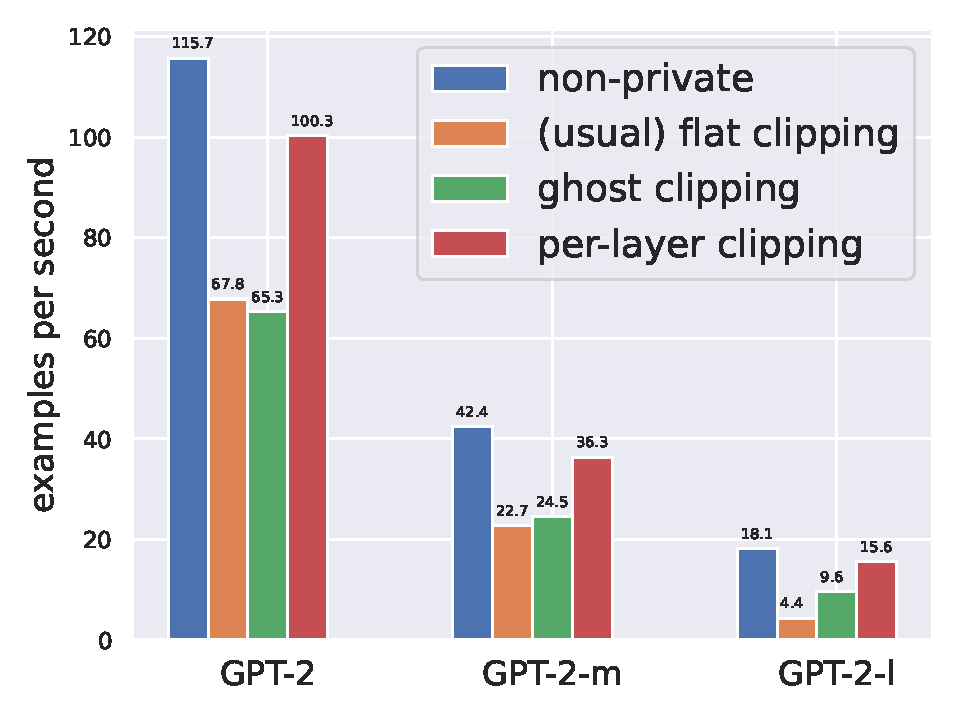
\includegraphics[width=0.95\textwidth]{files/fig/profile_v2/throughput_100_default_fast_float.pdf}} \\
(b) Throughput
\end{minipage}
\end{center}
\caption{
Private learning with (adaptive) per-layer clipping can be almost as efficient as non-private learning (the throughput gap is less than 15\% in this case).
}
\label{fig:gpt2runtime-breakdown}
\end{figure}

